\subsection*{1. Executar os diferentes servidores em uma máquina diferente da
máquina cliente.}
\addcontentsline{toc}{section}{1. Executar os servidores}

Os \textit{}{Batch Scripts} foram reescritos como \textit{Shell Scripts} com o intuito de serem executados tanto no Linux nativo (Manjaro Linux) quanto no \textit{Windows Subsystem for Linux} (WSL). Os scripts todos estão disponíveis no arquivo zipado, junto com os Batch Scripts


\subsubsection{1.1 - Servidor: executar o rmi.bat e depois o server.bat.}
\addcontentsline{toc}{subsection}{1.1 Execução do servidor}

Primeiramente foi executado o comando \textit{rmiregistry}, seguido pelo script \texttt{server.sh} para iniciar comunicação com o registro e o armazenamento das informações do servidor.

\vspace{2em}
\begin{minipage}{\textwidth}
    \hspace{-1em}
    \centering
    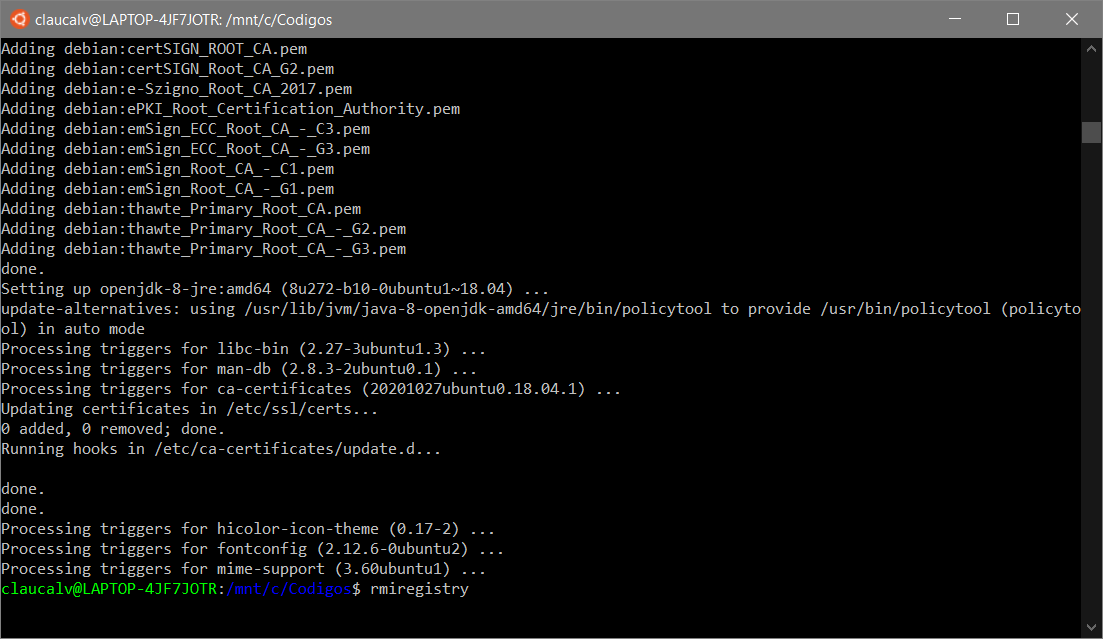
\includegraphics[scale=.35]{prints/rmiregistry.PNG}
    \hspace{1em}
    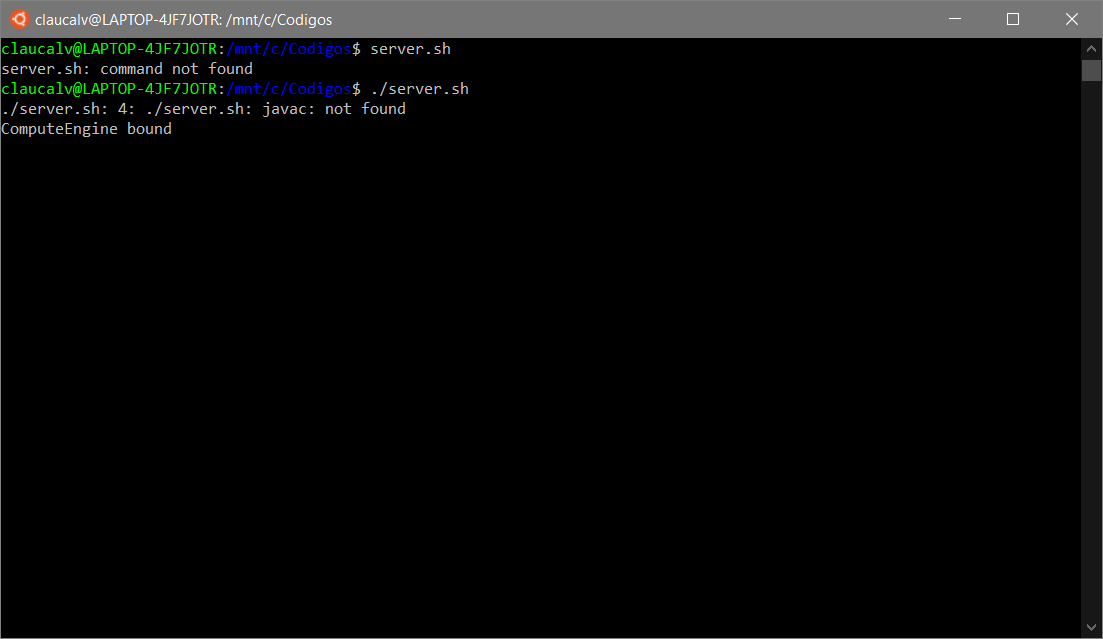
\includegraphics[scale=.35]{prints/server.PNG}
    \captionof{figure}{Execução do rmiregistry e do server}
    \label{threadspng}
    \hspace{1em}
\end{minipage}
\vspace{0.5em}


\subsubsection{1.2 - Cliente: executar o client.bat. Discorra sobre os tempos obtidos na
execução de forma remota e local.}
\addcontentsline{toc}{subsection}{1.2 Execução do client}

Foi feita a execução do arquivo \textit{client.sh} adaptado do \textit{client.bat} para execução no WSL.

\vspace{2em}
\begin{minipage}{\textwidth}
    \hspace{-1em}
    \centering
    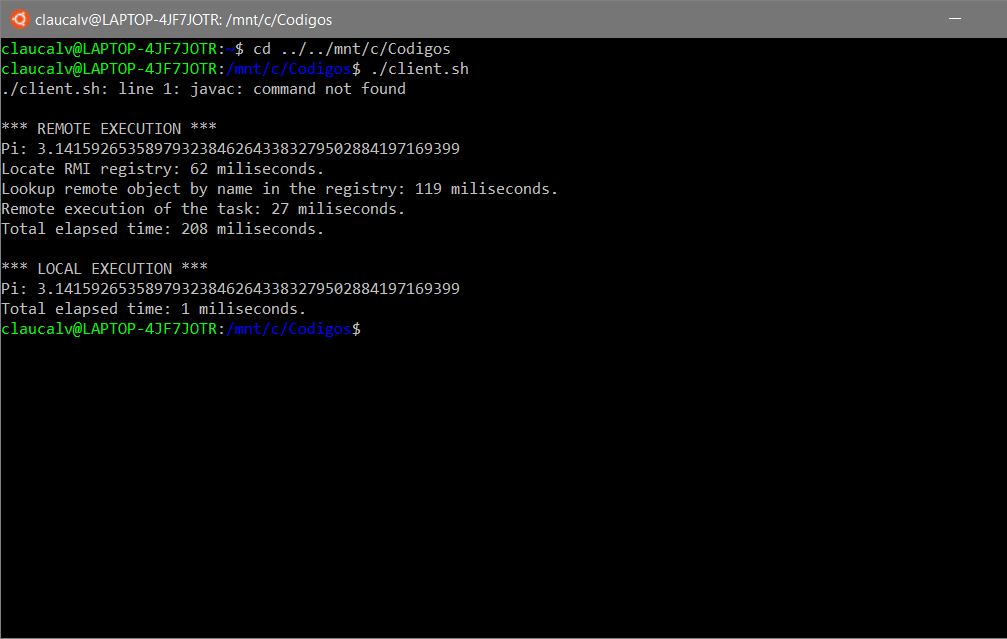
\includegraphics[trim= 0 150 250 0, clip, scale=.4]{prints/client.PNG}
    \captionof{figure}{Execução do cliente}
    \label{threadspng}
    \hspace{1em}
\end{minipage}
\vspace{0.5em}


\subsection*{2. Executar a classe \textit{serialization.SerialObject} com os parâmetros adequados (nome de arquivo e operação).}
\addcontentsline{toc}{section}{2. Execução da serialização}



\vspace{2em}
\begin{minipage}{\textwidth}
    \hspace{-1em}
    \centering
    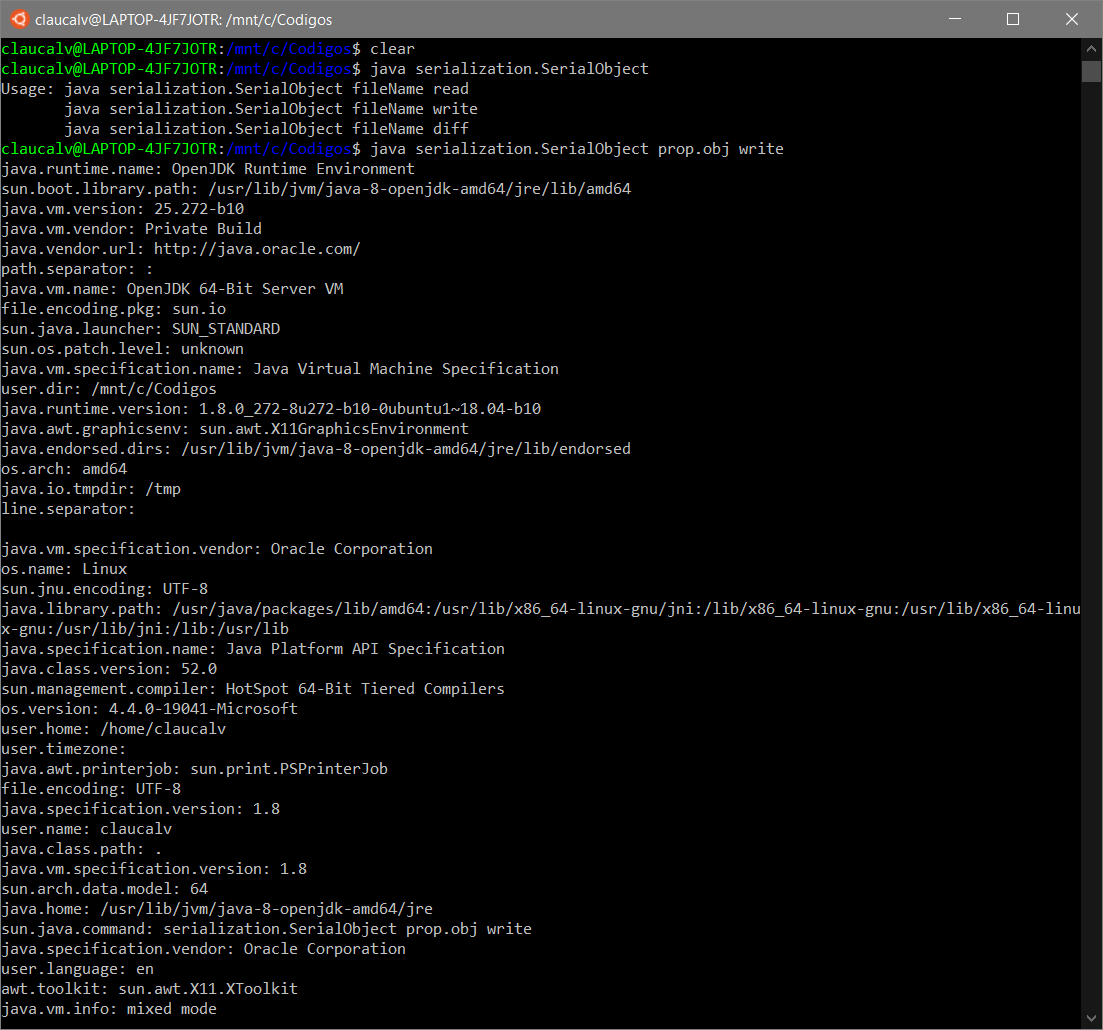
\includegraphics[scale=.35]{prints/serial1.PNG}
    \hspace{1em}
    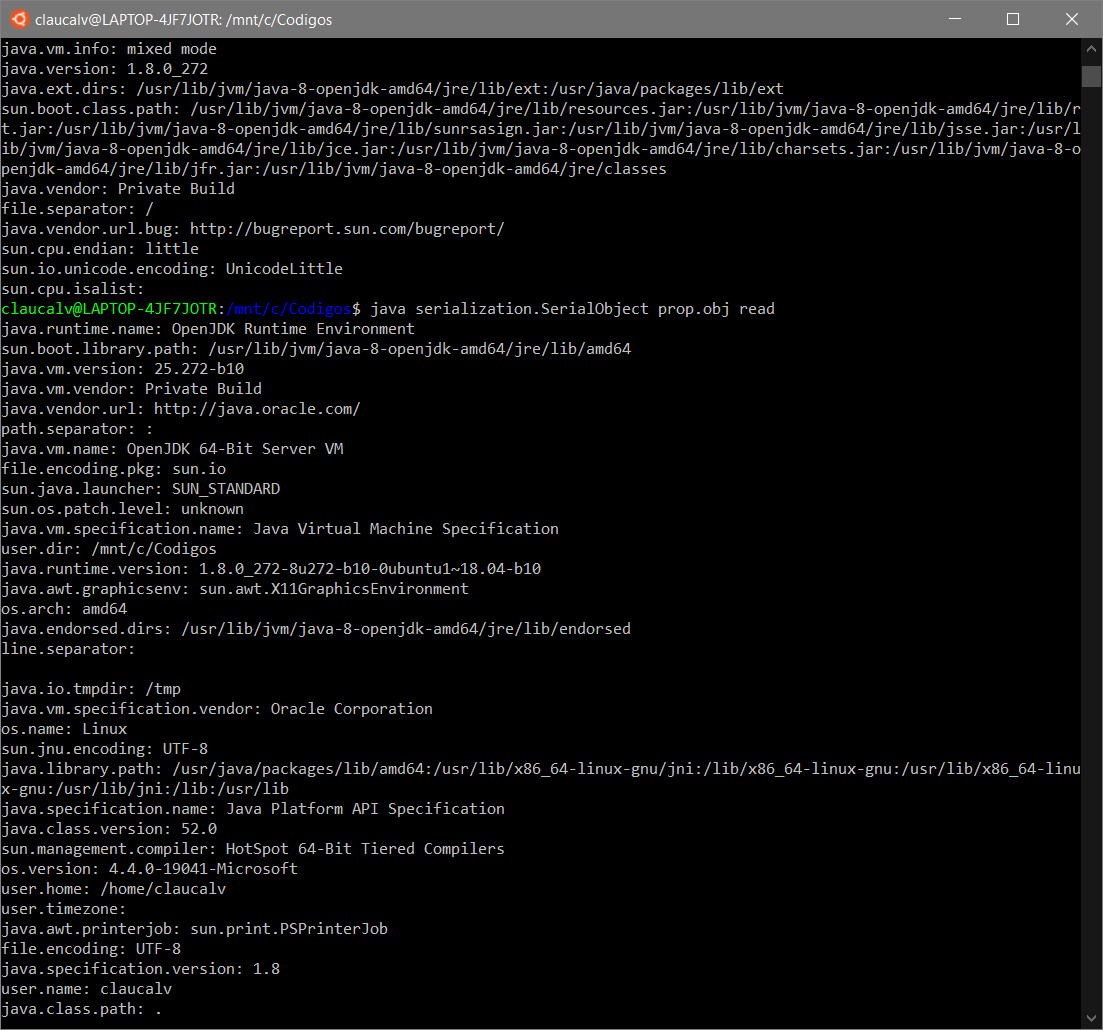
\includegraphics[scale=.35]{prints/serial2.PNG}
    \hspace{1em}
    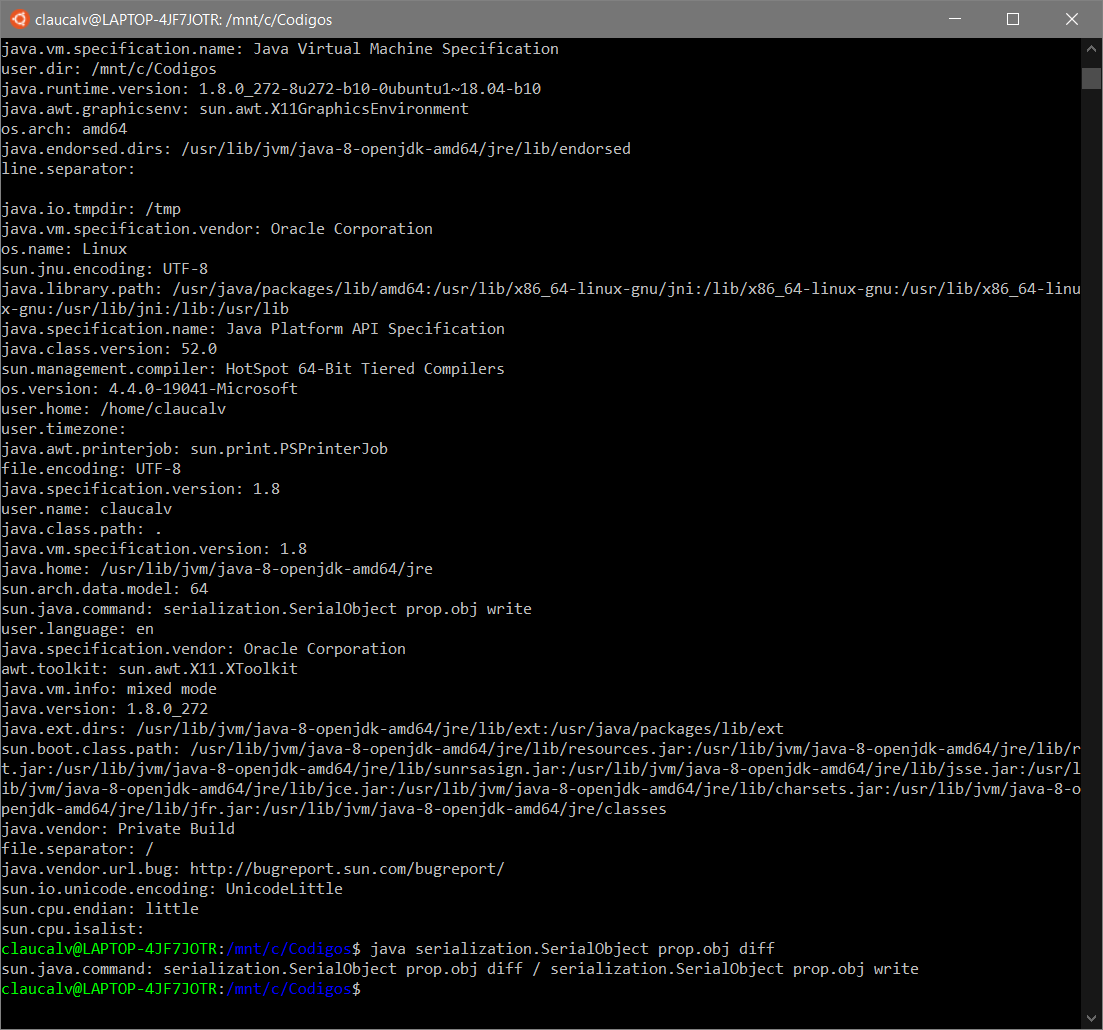
\includegraphics[scale=.35]{prints/serial3.PNG}
    \captionof{figure}{Execução do SerialObject}
    \label{threadspng}
    \hspace{1em}
\end{minipage}
\vspace{0.5em}

\subsubsection{2.1 - Qual o papel de cada operação (write, read e diff)?}
\addcontentsline{toc}{subsection}{2.1 Diferenças de operação}

A operação \textit{write} grava em arquivo o objeto \textit{System.properties}. A operação \textit{read} recupera o arquivo \textit{properties} (uma \textit{hashtable}) e imprime na tela. A operação \textit{diff} faz a diferença entre o arquivo e o \textit{System.properties} atual.

\subsection*{3. Implementar um sistema cliente-servidor em que o cliente envia seu objeto \textit{Properties} a um servidor por meio de \textit{socket}. O servidor compara o objeto enviado com seu próprio \textit{Properties} e devolve o resultado da operação \textit{diff} ao cliente, que é impresso na tela}
\addcontentsline{toc}{section}{3. Implementação cliente-servidor}

\vspace{-0.5em}
\begin{minipage}{\textwidth}
  \hspace{-1em}
  \centering
  \lstinputlisting[language=Java]{codigos/serialization/SerialObjectServer.java}
  \captionof{figure}{Implementação do servidor da serialização}
  \label{prog1}
  \hspace{1em}
\end{minipage}
\vspace{0.5em}

\vspace{-0.5em}
\begin{minipage}{\textwidth}
  \hspace{-1em}
  \centering
  \lstinputlisting[language=Java]{codigos/serialization/SerialObjectClient.java}
  \captionof{figure}{Implementação do cliente da serialização}
  \label{prog1}
  \hspace{1em}
\end{minipage}
\vspace{0.5em}

\vspace{2em}
\begin{minipage}{\textwidth}
    \hspace{-1em}
    \centering
    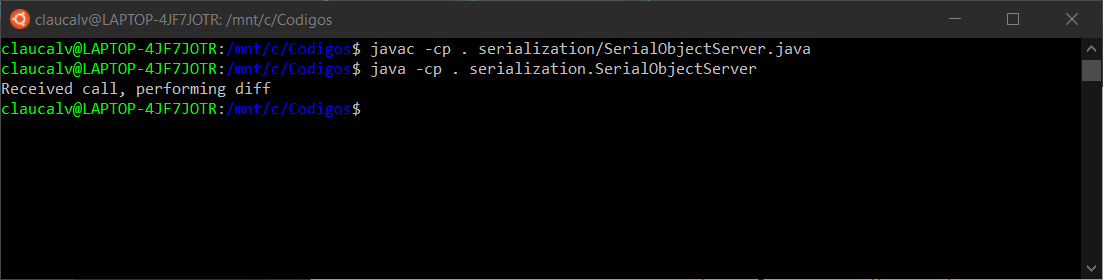
\includegraphics[scale=.35]{prints/serial_server.PNG}
    \hspace{1em}
    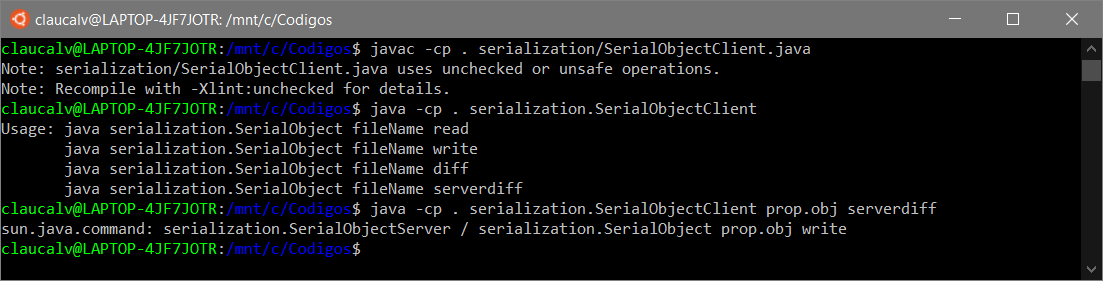
\includegraphics[scale=.35]{prints/serial_client.PNG}
    \captionof{figure}{Execução do servidor e cliente da serialização}
    \label{threadspng}
    \hspace{1em}
\end{minipage}
\vspace{0.5em}